\section{Data representation}
Inside databases and datasets we can identify:
\begin{itemize}
\item \textbf{Instances} $\to$ observations/cases/records that represent atomic elements of information
\item \textbf{Attributes} $\to$ variables/features that measure aspects of an instance. Each instance has a certain number of attributes
\item \textbf{Concepts} $\to$ things that can be learned inside the data
\end{itemize}

\subsection{Attribute types}
Data types are not only important for our understanding but some algorithms work better with a certain type of data : make it easier to make adequate comparisons for example. \\
Knowing the data type is also important the check for \textbf{valid values} and deal with \textbf{missing values}.
\begin{description}
\item[Numeric attributes]\hfill\\
\begin{itemize}
\item Real-valued or integer-valued domain
\item Interval-scaled when only differences are useful $\to$ temperature
\item Ratio-scaled when only rations are meaningful $\to$ age
\end{itemize}
Numerical attributes are \textbf{ordered} and measured in fixed units.\\
Zero point is only defied for \textbf{ratio attributes}.\\
Can be divided into \textit{discrete or continuous}.
\item[Categorical attributes]\hfill\\
\begin{itemize}
\item Set-valued domain composed of a set of symbols
\item \textit{Nominal}\\ When only equality is meaningful
Values are distinct symbols that serve as labels. No relation is implied among nominal values and only equality test can be performed.
\item \textit{Ordinal}\\When both equality and inequality are meaningful. As in the nominal case, also here talking about \textbf{difference} doesn't make sense.
\end{itemize}
\item[Binary attributes]\hfill\\
Represented by either 0/1

\end{description}
Sometimes the same attribute can be either considered \textbf{nominal} or \textbf{ordinal} : \texttt{if age == young AND ...} is nominal whereas \texttt{if age < presbyopic AND...} is ordinal.\\

\subsection{Missing values}
Many databases present \textbf{missing values} . The nature of missing values is very broad and must be understood : it can be due to faulty equipment, incorrect measurements, censored or anonymous data  ecc...\\
Missing values can have their own importance ( ex: a missing test ) but in that case is should have its own coding.It is important to find out \textbf{why} the value is missing : if the absence of value has some significance then \textbf{'missing'} is a separate value; if it does not it must be treated in a \textbf{special way}.
Usually missing values are indicated by \textbf{out of range } entries, \textbf{Nan} or \textbf{special values}. \\
\subsubsection{Missing values - types}
There are three types of missing values:
\begin{itemize}
\item \textbf{MCAR - Missing completely at random}\\
The distribution of an example having a missing value for an attribute \textbf{does not depend on either the observed data or the missing data} (doesn't give you a hint on why it is missing). Example : people omitting geolocation on Twitter.
\item  \textbf{MAR - Missing at random}\\
The distribution of an example having a missing value for an attribute \textbf{depends on the observed data, but does not depend on the missing data} ( the missing is not related to the missing data but to some observed data) . Example : people not giving out how much they earn not because of the amount but because they don't want to.
\item \textbf{NMAR - Not missing at random}\\
The distribution of an example having a missing value  \textbf{depends on the missing value}.
Example : people not telling they salary because of their position ( so related to the amount).
\end{itemize}
\subsubsection{Missing values - solutions}
When dealing with missing values one should always try to find out 
\begin{itemize}
\item Why data is missing
\item Distribution of missing data
\end{itemize}
Then different methods can be applied to deal with missing values depending on the type of missing value:
\begin{itemize}
\item \textbf{Discard} examples with missing values\\
Simplest approach which allows to used \textbf{unmodified data}. This method should be used only if we have \textbf{lots of data} and with \textbf{low number} of missing values because otherwise \textbf{bias} can be introduced.
\item \textbf{Fill in manually} missing values
\item \textbf{Convert into new value}\\
Using a special value just for the missing value one then you can use a boolean attribute to tell if it is missing or not ( increases difficulty of data mining process!)
\item \textbf{Imputation}\\
Assign a value to the missing one based on the rest of the dataset (mean/mode substitution, dummy variable imputation, regression...)
\end{itemize}
Some methods : 
\begin{itemize}
\item \textbf{Listwise deletion}\\
This way you only analyse cases with available data on each variable. This can reduces the number of available data greatly and should only be used with MCAR types in order to not \textbf{introduce bias}
\begin{figure}[H]
  \centering
  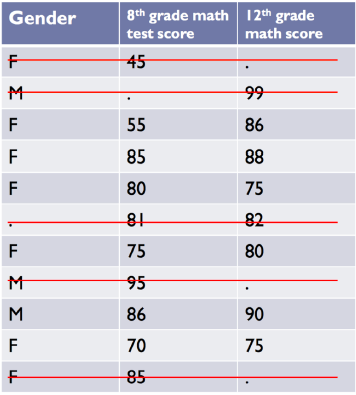
\includegraphics[width=.4\linewidth]{listwise}
\end{figure}
\item \textbf{Pairwise deletion}\\
This way examples are deleted only if considering that specific attribute ( say you are considering the Gender attribute then you only discard row 5). The method keeps as many cases as possible for each analysis but does not allow for comparison as the sample size can vary.
\begin{figure}[H]
  \centering
  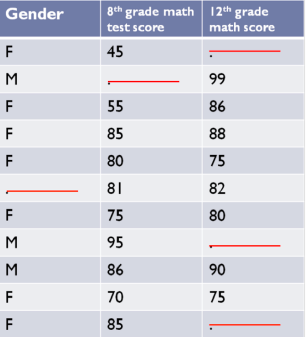
\includegraphics[width=.4\linewidth]{pairwise}
\end{figure}
\item \textbf{Imputation}\\
Imputation extracts a model from available data. It is suitable for MCAR and MAR ( to a lesser extend) but not for NMAR ( for NMAR we need to go back to the source of the data to obtain more information). There a several imputations methods like:
\begin{itemize}
\item \textbf{Mean/mode substitution}\\
Replace the missing values with the mean/mode . This allows to use the \textbf{complete case analysis} methods but \textbf{reduces variability}
\item \textbf{Dummy variable control}\\
Create an indicator for missing value (1 = missing, 0 =not missing) and impute missing values to constant (such as the mean). Then you include the missing indicator in the algorithm. Unfortunately results in \textbf{biased estimates} 
\item \textbf{Regression}\\
Replaces values with predicted values from a regression equation.\\
Otherwise you can choose to \textbf{not impute} by simply using the default policy of the data mining methods ( if one is present!)
\end{itemize}
\end{itemize}

\subsection{Inaccurate values}
Inaccurate values can happen for many reasons. For example data being collected but not for mining purposes : in this case an error does not affect the original purpose of the data ( for example age of customer). Errors can be of many types :
\begin{itemize}
\item \textbf{Typographical errors in nominal attributes}
\item \textbf{Typographical errors in numeric attributes}
\item \textbf{Deliberate errors} (invent answers for example)
\end{itemize}
Other than the \textbf{probabilistic view} of data ( distribution,mean...) the more common way to view data is the \textbf{geometric view}.
\begin{figure}[H]
  \centering
  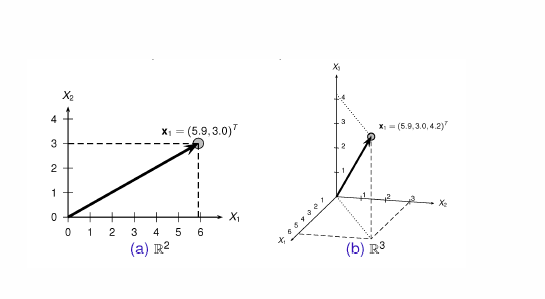
\includegraphics[width=.4\linewidth]{geomview}
\end{figure}
\begin{figure}[H]
  \centering
  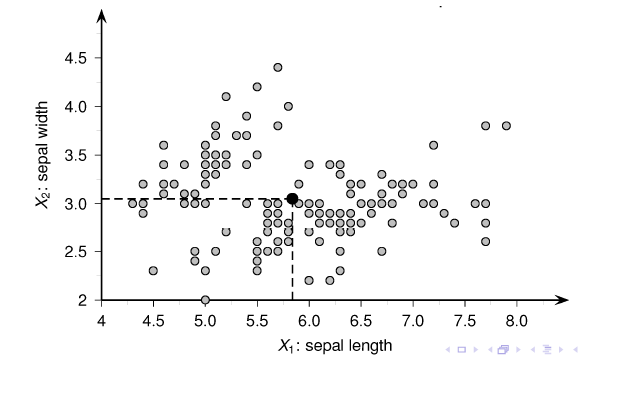
\includegraphics[width=.4\linewidth]{geomview2}
\end{figure}

\subsection{Data format}
There are not many data formats (neither for storing nor for data exchange) as most commercial tools have their own format.Most tools import \textbf{excel} and \textbf{CSV - comma separated values} files. Over the years many \textbf{standardization formats} have been proposed :
\begin{itemize}
\item \textbf{Attribute Relation File Format (ARFF)}\\
Very popular ,rising since Java ML libraries have been made available. With the \texttt{@attribute} you can declare an attribute name and specify its \textbf{type} ,\textbf{possible values} or \textbf{range}. This allows for \textbf{cross checking} if the data is correct.\\
ARFF also supports \textbf{sparse representation} $$ 0,26,0,0,0,0,63,0,0 \to \{1 \quad 26, 6 \quad 63,10\} $$
Missing values in ARFF are \textbf{'?'}
\begin{figure}[H]
  \centering
  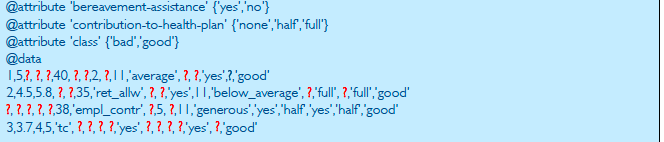
\includegraphics[width=.5\linewidth]{arffmissing}
\end{figure}
\item \textbf{Dataset Publishing Language (DSPL)}\\
Open format from Google. Simply add an XML file to an existing CSV file 
\end{itemize} 

\subsection{Model representation}
The \textbf{Predictive Model Markup Language} is an XML-based markup language created to provide a way for applications to define models related to predictive data mining.The goal is to \textbf{share} models between applications using different components ( data dictionaries, data transformations,mode,data mining schema,target,output)